%----------------------------------------------------------------------------------------
% Analisi del contesto
%----------------------------------------------------------------------------------------

\documentclass[10pt]{softeng} % Document font size and equations flushed left

%----------------------------------------------------------------------------------------
%	ARTICLE INFORMATION
%----------------------------------------------------------------------------------------

\Phase{Inception - I iterazione} % Additional notes (e.g. copyright, DOI, review/research article)

\DocumentTitle{Analisi del contesto e studio di fattibilit\`a} % Article title

%----------------------------------------------------------------------------------------

\begin{document}

\startofdocument{}

\section{Collocazione del progetto}

La nostra societa si impegna a realizzare un sistema informatico di home banking, compatibile con lo standard OBP.
Obiettivo del progetto \`e la realizzazione di un software di Home Banking, i cui utenti sono unicamente persone fisiche.
Il nostro software cerca di fornire all'utente un mezzo semplice ed intuitivo per poter effettuare le operazioni bancarie quotidiane senza doversi recare alla banca.
Un software di Home Banking deve (idealmente) permettere all'utente di effettuare via internet tutte le operazioni che pu\`o normalmente effettuare allo sportello della sua banca.
Il sistema home banking \`e accessibile tramite un semplice browser web, e non richiede software aggiuntivo.
D'altronde l'utilizzo di tecnologie come TLS e HTTPS permette di rendere sicura la connessione per poter trasmettere le informazioni sensibili in modo sicuro.

% intenzione progetto, collocazione

\section{Analisi del contesto}
Un sistema home banking \`e un sistema informatco che permette agli utenti di effettuare le operazioni bancarie autonomamente, senza recarsi alla banca.
In genere i sistemi di home banking presenti sul mercato forniscono uno o pi\`u tipi d'iterfaccia utente:
\begin{enumerate}
    \item Interfaccia web, con accesso tramite un browser web
    \item Applicazione per una piattaforma mobile come Android o ios.
    \item Applicazione per personal computer.
\end{enumerate}
Attualmente il terzo tipo di interfaccia non si incontra pi\`u nei sistemi home banking, ma si impiega principalmente negli ambienti che richiedono le caratteristiche che una \emph{web app} non pu\`o fornire. La maggioranza dei sistemi di \emph{trading online} professionali forniscono un software apposito.
%TODO glossario trading online

%TODO glossario Applicazione Web, Web-app

Data la natura sensibile dei dati bancari, tutti i sistemi di home banking devono unsare un canale sicuro per trasferire i dati tra il dispositivo dell'utente e i sistemi della banca.

Le applicazioni web usano protocolli sicuri come TLS e HTTPS per proteggere i dati sensibili.
%TODO glossario TLS, HTTPS

Con lo sviluppo delle tecnologie internet banking alcune banche hanno scelto di abbandonare l'infrastruttura tradizionale e diventare \emph{Banche Online}. Questo approccio permette di talgiare le spese e offire ai clienti offerte pi\`u vantaggiose.
%allora le banche online le dobbiamo mettere mi sa, se no caviamo questa parte
%se le mettiamo allora dobbiamo modificare la parte di registrazione
%TODO glossario banca online

Chiamiamo ``utente registrato (al sistema di Home Banking della banca X)'' una persona fisica titolare di un account di Home Banking all'interno del sistema di una particolare banca, e che quindi abbia fornito informazioni anagrafiche e di contatto, e eventualmente informazioni non obbligatorie sulla sua condizione economica e famigliare.

Chiamiamo ``utente titolare di un conto corrente'' un utente registrato presso la banca X che abbia ultimato la procedura di autenticazione della suddetta banca.

Il bonifico \`e un trasferimento di denaro da un conto corrente a un altro.
Un utente titolare di un conto corrente pu\`o effettuare bonifici dal suo conto corrente.
Distinguiamo due tipi di bonifici:
\begin{itemize}
	\item Bonifico Italia se il conto corrente destinatario \`e aperto presso una banca italiana.
	Per effettuare un Bonifico Italia \`e necessario conoscere nome, cognome, indirizzo e codice IBAN del destinatario.
	\item Bonifico SEPA se il conto corrente destinatario \`e aperto presso una banca europea. Per effettuare un Bonifico SEPA \`e necessario conoscere anche il codice BIC/SWIFT della banca del destinatario \cite{bonifico_unicredit}.
\end{itemize}
Poich\'e la maggioranza dei pagamenti che una persona deve effettuare (tasse, bollette, ricariche, etc.) avvengono tramite bonifico, utenti di un sistema di Home Banking ritengono utile la possibilit\`a di effettuare pagamenti di un certo tipo tramite ``maschere specializzate'', che facilitino la compilazione dei dati e aiutino l'utente a evitare errori.

\subsection{Conti di deposito}

Un conto di deposito \`e una tipoligia di contratto bancario.
A differenza del conto corrente il conto di deposito non permette maggior parte delle operazioni bancarie.
In genere un conto di deposito prevede solamente operazioni di prelievo e versamento.
Il conto di deposito pu\`o essere di due tipi:
\begin{enumerate}
    \item Libero - Un conto di deposito libero permette di ritirare qualsiasi quantit\`a di denaro in qualunque momento.
    \item Vincolato - Un conto di deposito vincolato prevede una scadenza, entro la quale il ritiro dei soldi prevede una penalit\`a. In genere la penalit\`a consiste nella perdita totale degli interessi. Le scadenze tipiche sono da 1 mese a 3 anni.
\end{enumerate}


% TODO scrivere qualcosa o togliere

\subsection{Portafoglio fondi}

Nel 1999 \`e stato publicato il \emph{ "Nuovo Regolamento Consob di attuazione del Testo Unico dei mercati finanziari"} che stabilisce le modalit\`a di compravendita si strumenti finanziari come:
\begin{enumerate}
    \item Azioni
    \item Obbligazioni
    \item Titoli statali
\end{enumerate}

Nel campo di \emph{trading online} al primo posto sono le applicazioni per personal computer, perch\`e sono in grado di offrire un un interfaccia pi\`u flessibile e tempi di risposta migliori rispetto a un applicazione web. In particolare devono mostrare grafici di andamento dei vari titoli in tempo reale per fornire all'utente una panoramica ampia.

Spesso le banche che forniscono servizi di \emph{trading online} mettono a disposizione dei contratti di conto corrente specifici per facilitare il \emph{trading}.

Le norme che regolano l'acquisto di azioni e le procedure necessarie per acquisire dati aggiornati sull'andamento dei titoli esulano dalla portata di questo progetto, ricadendo nell'area di competenza del \emph{trading online}, e non dell'Home Banking.

% TODO espandere: fare tutto \`e infattibile, riduciamo roba da fare
% al max gli utenti vedono i fondi e possono venderli

\subsection{Certificati di deposito}
%paro paro da wikipedia

I certificati di deposito sono titoli vincolati e trasferibili che attribuiscono al possessore il diritto al rimborso del capitale più un interesse.
In genere questi titoli hanno una scadenza e vengono rimborsati al termine di essa.

Ce ne sono 3 tipi:
\begin{enumerate}
    \item Certificati di deposito a tasso fisso: prevedono un tasso di interesse fisso stabilito prima dell'emissione.
    \item Certificati di deposito a tasso variabile:Il tasso di interesse varia a determinate scadenze temporali seguendo i tassi di mercato.
    \item Certificati di deposito zero-coupon: a differenza dei primi due non prevedono interessi.
\end{enumerate}

A volte i certificati di deposito sono soggetti a vincoli aggiuntivi, per esempio in alcuni casi prevedono un periodo entro la fine del quale non possono essere rimborsati.

\subsection{Legislazione taliana}

La Banca d'Italia si occupa di esercitare ``l'attivit\`a di vigilanza sulle banche'', e ``ha funzioni di controllo in materia di antiriciclaggio'' \cite[Funzioni]{banca_italia}.

% TODO espandere: cosa serve

\section{Fattibilit\`a}

L'analisi del mercato mostra che attualmente non \`e disponibile alcun \emph{framework} di \emph{internet banking} compatibile con lo standard OBP.
La nuova legislazione rende obbligatorio lo standard OBP per tutte le banche che forniscono serivzi online.
La percentuale delle banche che usano i sistemi gia aderenti allo standard \`e ancora molto bassa.
%vogliamo dare una percentuale a buffo?
E anche in quei casi si tratta spesso di un software costruito su misura per una specifica banca.
Quindi visto che la nuova legislazione rende obbligatorio lo standard OBP si prevede che molte banche si troveranno senza un sistema di \emph{banking online}.
Sopratutto le banche piccole avranno bisogno di un sistema ``prefabbricato'', non avendo un ampio budget per sviluppare un sistema personalizzato \emph{from scratch}.
La nostra societa vuole cogliere l'occasione di colmare questa lacuna.
Inoltre la consideriamo un ottima occasione per guadagnare un posto in questo mercato altamente competitivo e redditizio.

\section{Fattibilit\`a}


Per motivi di sicurezza, legislativi, burocratici e tecnologici non \`e possibile effettuare ogni operazione via internet.
Un sistema di Home Banking effettuer\`a quindi un sottoinsieme proprio di queste operazioni.


Le banche target del nostro prodotto sono banche di taglia piccola, che a seguito dell'entrata in vigore dello standard OBP si troveranno sprovviste di sistema informatico. Il nostro prodotto permette loro di effettuare la transizione senza subire \emph{downtime}.

Definiamo il nostro software ``Small Bank Friendly'' in quanto:
\begin{itemize}
    \item Il software non viene sviluppato ``from scratch'' individualmente per ogni cliente, ci\`o riduce notevolmente il costo unitario.
    \item Il proggetto parte con l'idea di separare ed isolare le componenti rendendo il sistema adatto al deployment su cloud, evitando l'acquisto di hardware aggiuntivo.
    \item Il supporto per la banca \`e fornito dalla nostra societ\`a.
    \item Il supporto per gli utenti \`e fornito dalla nostra societ\`a (o partner di essa)
\end {itemize}

Questa impostazione permete al prodotto di essere competitivo dal punto di vista del prezzo, i costi di servizio di supporto vengono distribuiti fra pi\`u clienti. 



Dato che l'insieme delle funzionalit\`a core \`e relativamente piccolo e restringibile a piacere, si d\`a per scontato la fattibilit\`a.

Perch\'e lo sforzo di sviluppo sia ripagato \`e per\`o necessario che l'insieme di operazioni offerte dal sistema sia sufficientemente ampio da:
\begin{enumerate}
	\item soddisfare le esigenze della maggioranza degli utenti;
	\item essere generale al punto da fornire tutti i principali servizi di cui la banca che utilizza il software ha bisogno.
\end{enumerate}
L'effettiva fattibilit\`a viene quindi da una combinazione delle due considerazioni.


Attualmente la quasi totalit\`a banche dispongono di un sistema di Home Banking.
L'introduzione dello standard OBP rende per\`o tutti questi sistemi obsoleti.
Il nostro progetto soddisfa un mercato che avr\`a bisogno in tempi brevi di un nuovo sistema di Home Banking.
Inoltre un software di Home Banking modulare e facilmente personalizzabile pu\`o essere adattato alle esigenze di pi\`u banche con \emph{refactoring} minimo, e quindi a costi ridotti.

\subsection{Requisiti minimi}

Abbiamo individuato i seguenti requisiti minimi, che riteniamo essere sufficienti a soddisfare le necessit\`a di buona parte delle banche.

% TODO espandere e copiare da documento requisiti

\subsection{Fattibilit\`a economica}

Il mercato di software bancario \`e altamente competitivo e altamente redditizio.
Inoltre \`e estremamente difficile entrare a far' parte di questo mercato.
La nostra societa vuole sfruttare l'occasione del cambio di legislazione per colmare la lacuna che si verra a formare introducendo il nostro prodotto.
Naturalmente le altre societ\`a di sviluppo software staranno a loro volta attuando progetti simili.
L'unico modo di garantire la rentabilit\`a del prodotto \`e battere i concorrenti sul tempo.
Si tratta di un ambiente \emph{Winner Takes All}, dove il primo a mettere sul mercato un sistema che soddisfa i requisiti principali avr\`a il guadagno massimo.

% TODO inserire info su why il progetto pu\`o avere un guadagno

\section{Conclusioni}

Riteniamo sia fattibile, con le limitazioni indicate, realizzare un sistema di Home Banking all'avanguardia, manutenibile, espandibile e generale.

%----------------------------------------------------------------------------------------
%	CHANGELOG
%----------------------------------------------------------------------------------------

\section{Registro modifiche}

\subsection{Inception}

\subsubsection{I iterazione}

Prima stesura documento.

%----------------------------------------------------------------------------------------
%	REFERENCE LIST
%----------------------------------------------------------------------------------------

\printcustombibsmall{}

%----------------------------------------------------------------------------------------
%	FIGURES
%----------------------------------------------------------------------------------------

\begin{figure*}[hbt]
	\centering
	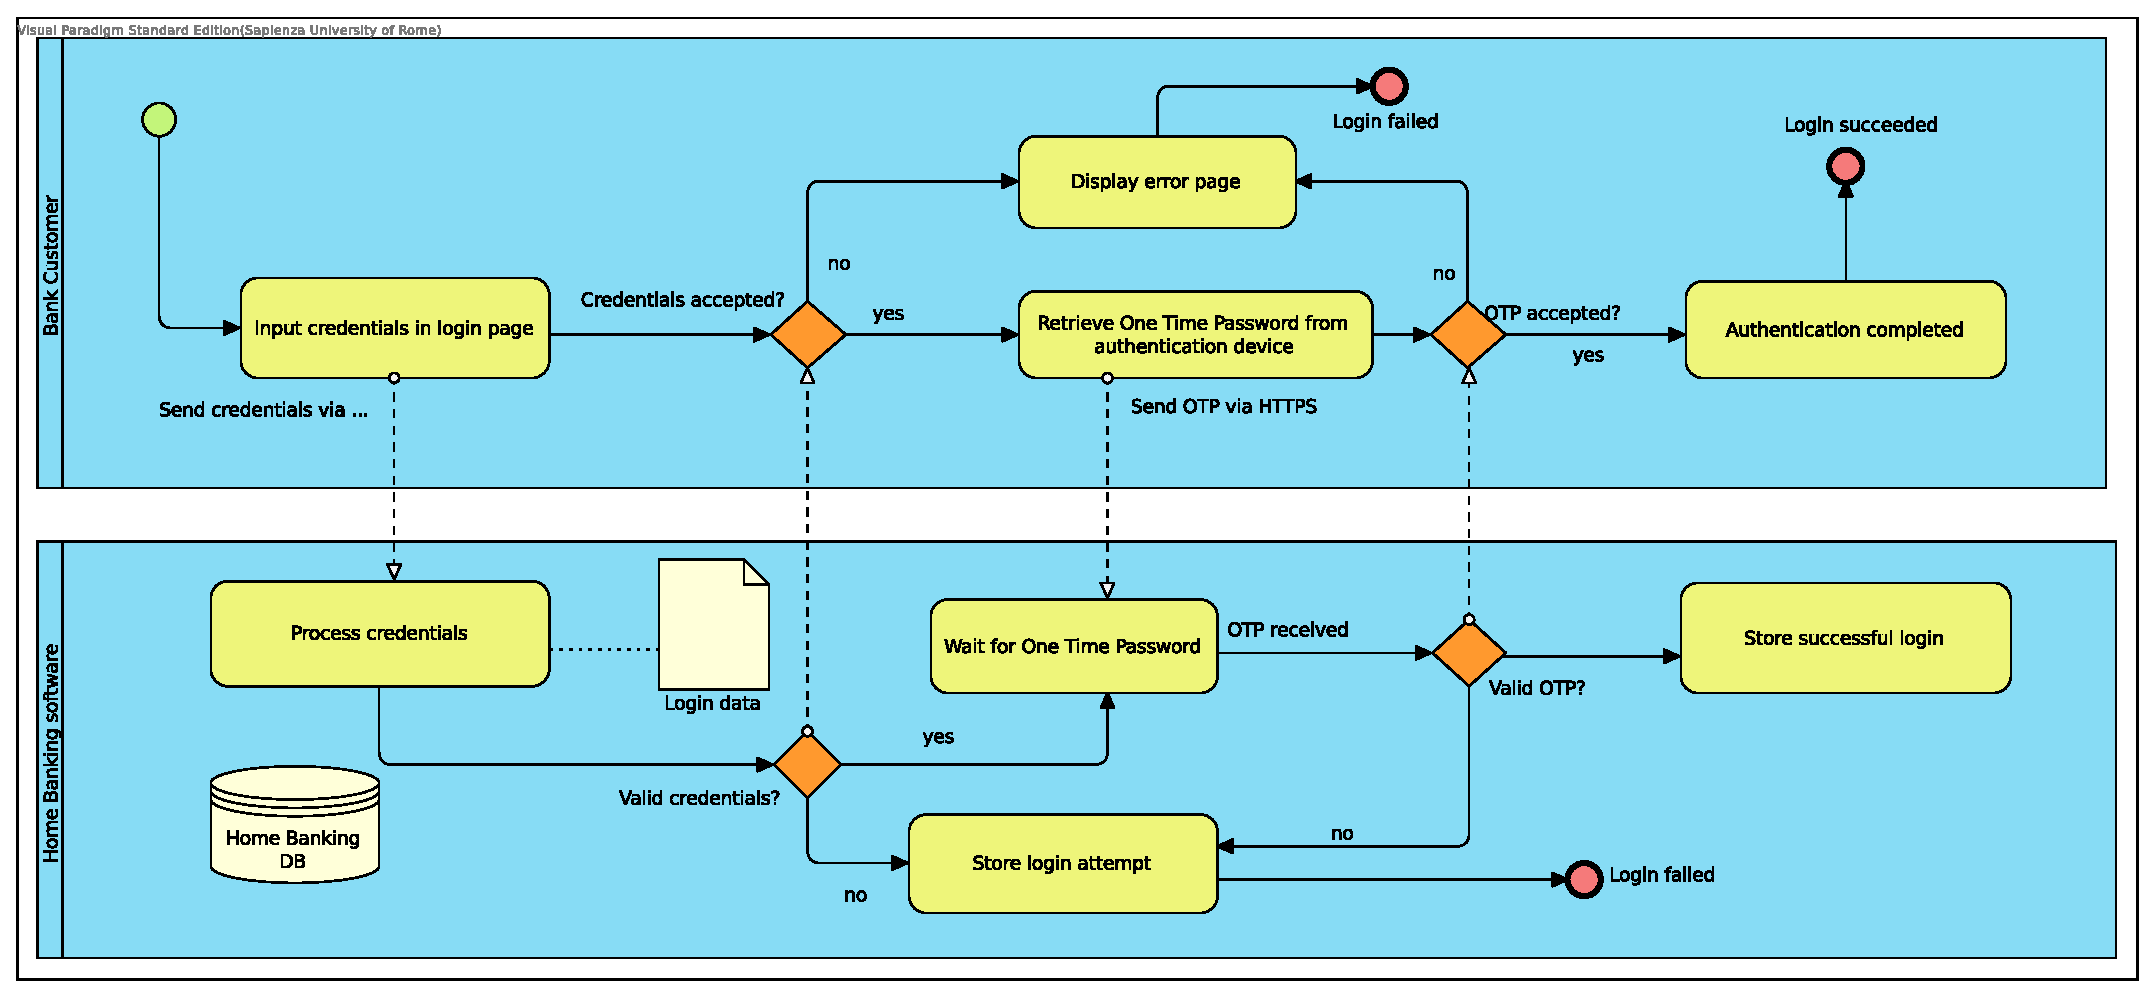
\includegraphics[width=\textheight, angle=90]{Images/Authentication.eps}
	\caption{Business case: procedura di autenticazione.}
	\label{fig:business_case_authentication}
\end{figure*}

\begin{figure*}[hbt]
	\centering
	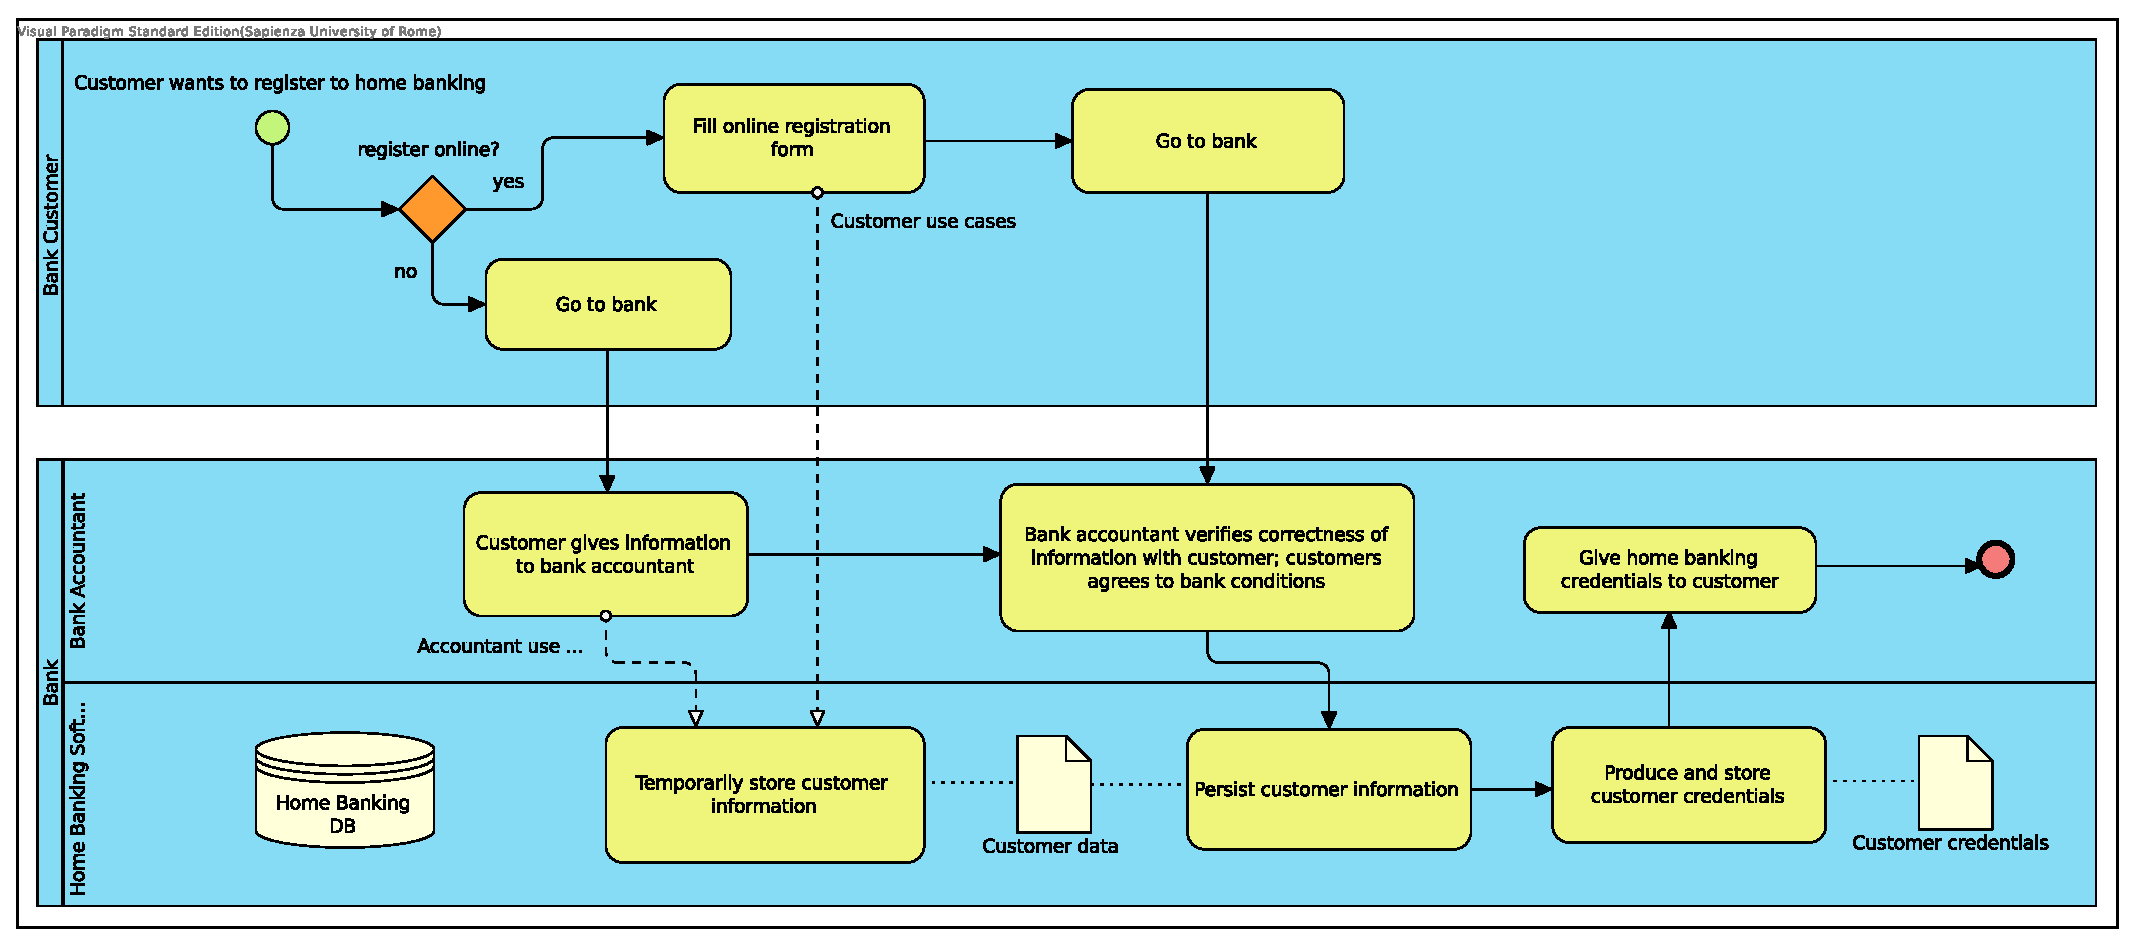
\includegraphics[width=\textheight, angle=90]{Images/Home_Banking_registration.eps}
	\caption{Business case: procedura di registrazione.}
	\label{fig:business_case_registration}
\end{figure*}

\begin{figure*}[hbt]
	\centering
	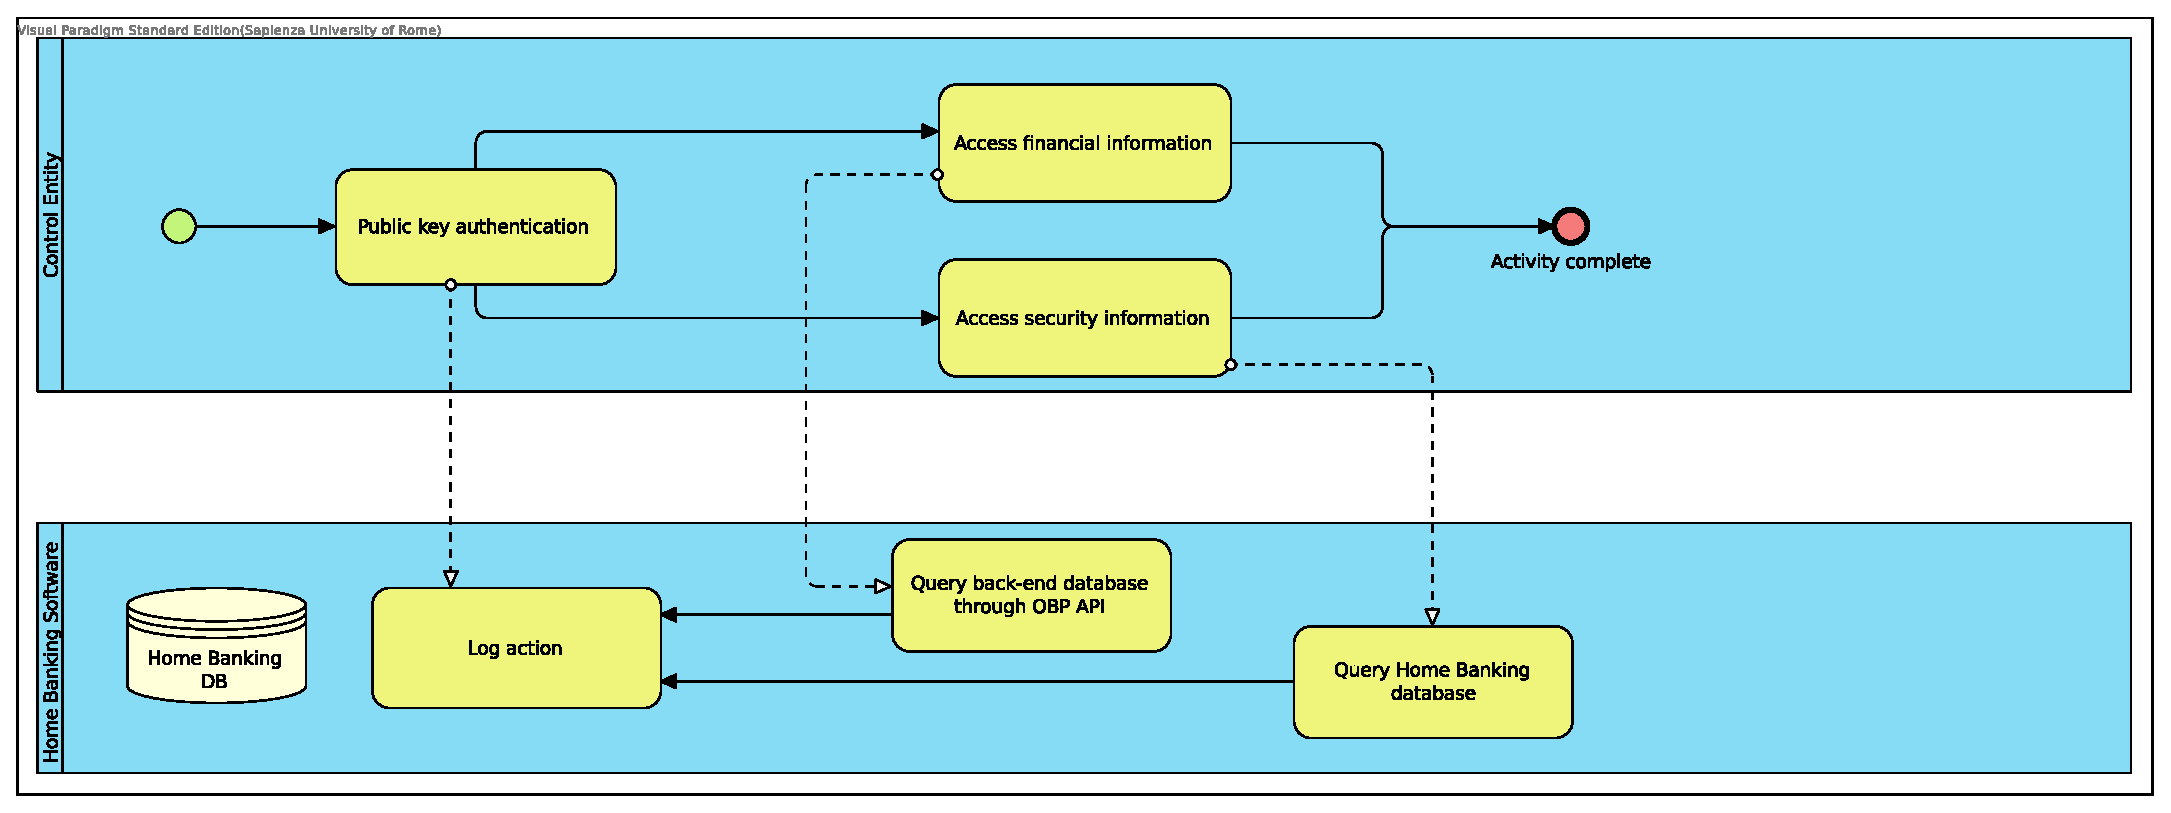
\includegraphics[width=\textheight, angle=90]{Images/Home_Banking_control_activity.eps}
	\caption{Business case: attivit\`a di controllo effettuata da enti responsabili.}
	\label{fig:business_case_control_activity}
\end{figure*}

\begin{figure*}[hbt]
	\centering
	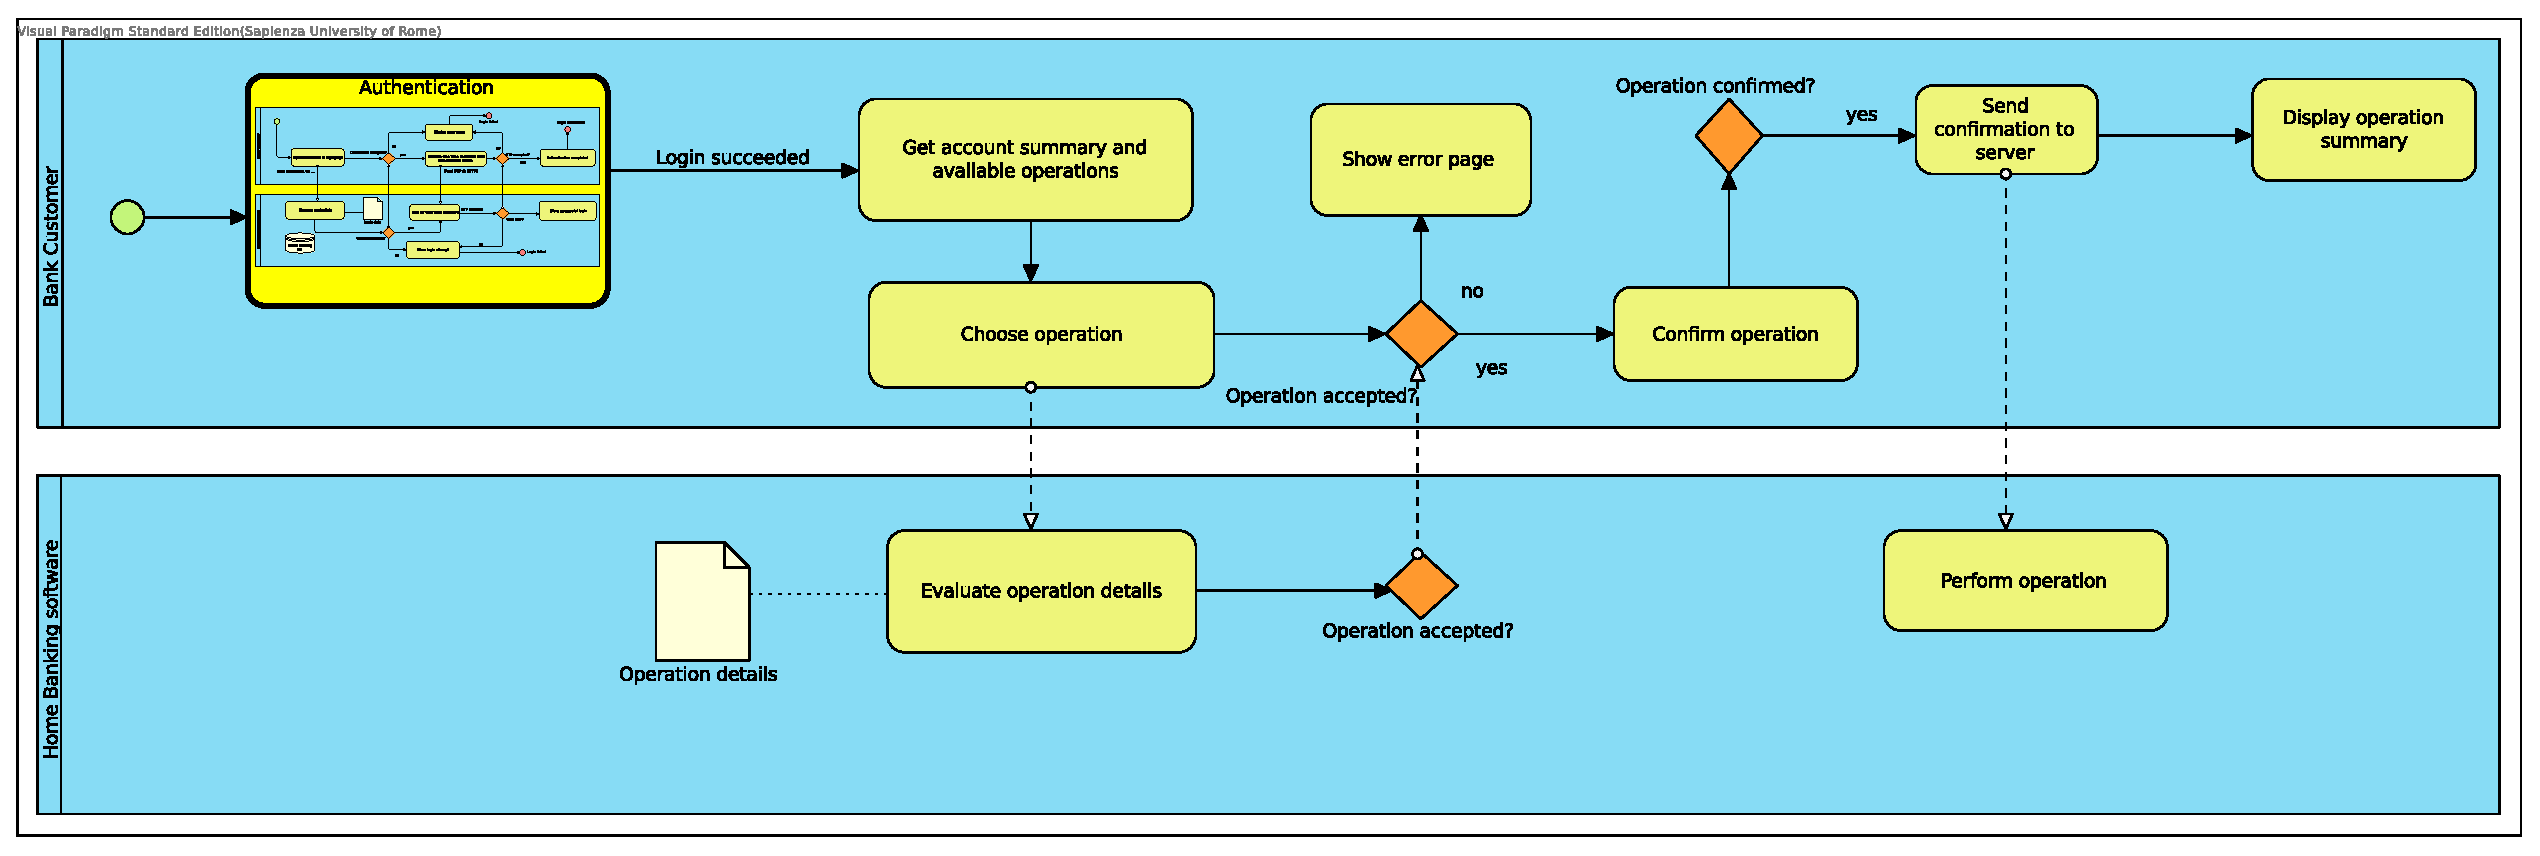
\includegraphics[width=\textheight, angle=90]{Images/Home_Banking_generic_action.eps}
	\caption{Business case: generica procedura di Home Banking effettuata da un utente del sistema.}
	\label{fig:business_case_generic_operation}
\end{figure*}

\end{document}
